%Version 3.1 December 2024

\documentclass[pdflatex,sn-basic]{sn-jnl}

\usepackage{graphicx}%
\usepackage{multirow}%
\usepackage{amsmath,amssymb,amsfonts}%
\usepackage{amsthm}%
\usepackage{mathrsfs}%
\usepackage[title]{appendix}%
\usepackage{xcolor}%
\usepackage{textcomp}%
\usepackage{manyfoot}%
\usepackage{booktabs}%
%\usepackage{algorithm}%
%\usepackage{algorithmicx}%
%\usepackage{algpseudocode}%
\usepackage{listings}%
%%%%

%% as per the requirement new theorem styles can be included as shown below
\theoremstyle{thmstyleone}%
\newtheorem{theorem}{Theorem}%  meant for continuous numbers
%%\newtheorem{theorem}{Theorem}[section]% meant for sectionwise numbers
%% optional argument [theorem] produces theorem numbering sequence instead of independent numbers for Proposition
\newtheorem{proposition}[theorem]{Proposition}% 
%%\newtheorem{proposition}{Proposition}% to get separate numbers for theorem and proposition etc.

\theoremstyle{thmstyletwo}%
\newtheorem{example}{Example}%
\newtheorem{remark}{Remark}%

\theoremstyle{thmstylethree}%
\newtheorem{definition}{Definition}%

\raggedbottom
%%\unnumbered% uncomment this for unnumbered level heads
\begin{document}

\title[Article Title]{Time vs. Duration: Lorentz-Consistent Minkowski Diagrams

\small\textit {(Preprint — April 2026)}}

\author*{\fnm{Ion} \sur{Vlad}}\email{contact@ionvlad.com}
\affil{\orgdiv{Independent Researcher}, \country{France}}

\abstract{The twin paradox is often presented as a consequence of time dilation and the relativity of simultaneity, yet its standard interpretation frequently relies on simplified Minkowski diagrams and ambiguous coordinate assignments that obscure the physical meaning of the turnaround event. This paper re-examines the paradox by constructing a Lorentz-consistent spacetime diagram in which inertial and accelerated phases are treated separately and coordinate assignments are preserved consistently across reference frames. We show that a single spacetime event is invariant under Lorentz transformation; different observers may assign different coordinates to that event, but they do not describe different physical occurrences \cite{malament1977, mtw1973}. The apparent contradiction arises not from simultaneity itself, but from conflating event identity with frame-dependent observation and from applying measurement transformations inconsistently after acceleration has ceased. This construction clarifies the operational meaning of simultaneity and demonstrates that the apparent paradox disappears once all measurements are analysed within a common comparison framework.}
 
\keywords{Time, Duration, Simultaneity, Paradox}

\maketitle

\section{Introduction}\label{sec1}
It is crucial to clarify the scope of this inquiry: this paper does not seek to refute the mathematical formalism or empirical predictions of Special Relativity, which remain robust and experimentally verified. In particular, we focus on two related issues:
	\begin{enumerate}
		\item the distinction between coordinate time and measured temporal intervals (duration)
		\item the interpretation of simultaneity and spacetime diagrams
	\end{enumerate}

This interpretation does not modify the formal structure of Special Relativity, but concerns only the ontological interpretation of coordinate time and event identity. Conceptual difficulties in Special Relativity persist despite the theory’s well-established mathematical structure. Among the most prominent are:
	\begin{itemize}
		\item the interpretation of spacetime diagrams
		\item the twin paradox
		\item the relativity of simultaneity
	\end{itemize}
These difficulties are often pedagogical rather than physical. As noted in standard treatments (e.g. Taylor and Wheeler 1992) \cite{taylor1992, french1968}, relativistic effects arise from well-defined transformation laws, yet their interpretation is frequently obscured by implicit classical intuitions.

We argue that several apparent paradoxes arise from conflating invariant event structure with frame-dependent coordinate assignments.
\section{Simultaneity – A Refined Framework}\label{sec2}
	\subsection{Geometric Analysis via Spacetime Diagrams}\label{subsec2_1}
		Consider the twin paradox scenario with a velocity of $v = 0.8c$ and a turnaround distance of 4 light-years. This configuration yields a coordinate time interval of $\Delta t_0$ = 5 years and a proper time interval of $\tau$ = 3 years. The corresponding spacetime representation is illustrated in Fig.~\ref{fig1}.
		\begin{figure}[h]
			\centering
			\makebox[\textwidth][c]{
        				
\includegraphics[width=1.3\textwidth]{figure1.png}
    			}
			\caption{Conventional schematic Minkowski representation of the twin paradox for v = 0.8c}\label{fig1}
		\end{figure}
As illustrated, the green dotted line of simultaneity passing through the turnaround point intersects the $ct$ axis at 1.8 years, not 3 years. This is because spacetime diagrams are typically not drawn to scale in order to simplify the representation. A Lorentz-consistent Minkowski diagram would appear as shown in Fig.~\ref{fig2}.
		\begin{figure}[h]
			\centering
			
\includegraphics[width=0.9\textwidth]{figure2.png}
			\caption{Lorentz-consistent Minkowski diagram illustrating the correct assignment of turnaround coordinates and simultaneity structure for $v = 0.8c$.}\label{fig2}
		\end{figure}
It is necessary to clarify how this diagram is constructed and what distinguishes it from conventional schematic representation.

  First, the spacing of the pink grid representing the frame S' is not uniform in Euclidean distance; instead, correct Minkowski grid spacing must satisfy:
		\begin{itemize}
			\item Equal increments in ct' correspond to: $ct-vx$ = constant increments
				\begin{equation*}
					ct = vx + \frac{k}{\gamma}
				\end{equation*}
			\item Equal increments in x' correspond to: $x-vct$ = constant increments
				\begin{equation*}
					x = vct + \frac{k}{\gamma}
				\end{equation*}
		\end{itemize}
The grid was rendered via a Python script. The source code is archived and accessible in the repository.

Second, it is essential to assign coordinates in a consistent manner:
		\begin{itemize}
			\item The event labeled T ($x = 4, ct = 5$) represents the turnaround point in frame S (does not exist in frame S')
			\item The event labeled T' ($x' = 4, ct'  = 5$) represents the turnaround point in frame S'. It is crucial to distinguish this from the event at ($x' = 2.4, ct' = 3$) to avoid conflation in the analysis.
			\item The event labeled P represents the projection of T' onto $ct$ axis (inertial frame)
			\item The event labeled P' represents the projection of T onto frame S'
		\end{itemize}
The points under consideration refer to the same physical event, expressed in different frames. \textbf{Once the Lorentz transformation has been applied to construct the S' grid (pink), the coordinates of the event in S must be preserved; applying the transformation again at the level of coordinates would amount to double counting.}

This potential error is illustrated by the simultaneity line of S' passing through the T. Read incorrectly, it may suggest that the event has coordinates ($x' = 0, ct' =3$) in S', which, when projected onto the $ct$ axis, would appear as ($x = 0, ct = 1.8$) (cf. the corresponding dotted lines in Fig.~\ref{fig1}). 

A simultaneity line in S' cannot be drawn through T, since T is not defined in that frame. However, T already represents the event in the S frame, with coordinates ($x = 4, ct = 5$), and cannot be reinterpreted within the same frame. The correct procedure is to retain the original S-coordinates and assign these values within the S' grid, yielding T' ($x' = 4, ct' = 5$)—turnaround in S'. This accounts for why T' does not possess the coordinates ($x' = 2.4, ct' = 3$). Projecting this point onto the $ct$ axis then gives P ($x = 0, ct = 3$), corresponding to the proper time recorded by the traveller during the outbound leg (3 years), in agreement with the predictions of Special Relativity.

To analyse an event from the traveller’s frame S', it must be expressed within that coordinate system. Upon projection onto S', T is identified as the same spacetime event, with coordinates P' ($x'=0, ct'=3$); therefore, a simultaneity line through T/P' in S' is not meaningful.
 The same construction applies to the return journey.

This construction clarifies the interpretation of simultaneity and the operational meaning of operationally invariant quantities in Special Relativity. While no inertial frame is physically preferred, comparisons between observers require the adoption of a common reference frame in which all quantities are expressed. In practice, this entails transforming all measurements into a chosen frame, analogous to expressing physical quantities in a common system of units.

The selected frame thus serves as a shared reference for comparison, without acquiring any fundamental status.

Simultaneity should not be conflated with visual appearance. In Fig.~\ref{fig2}, a single spacetime event is represented by different coordinate assignments in different reference frames, while its physical identity remains unchanged.

The differing simultaneity lines therefore reflect the frame-dependent manner in which events are described, and may be interpreted as observational slices through spacetime. Here, “observational slices” refers to frame-dependent hypersurfaces of constant coordinate time used to compare spatially separated events.
		\begin{figure}[h]
			\centering
			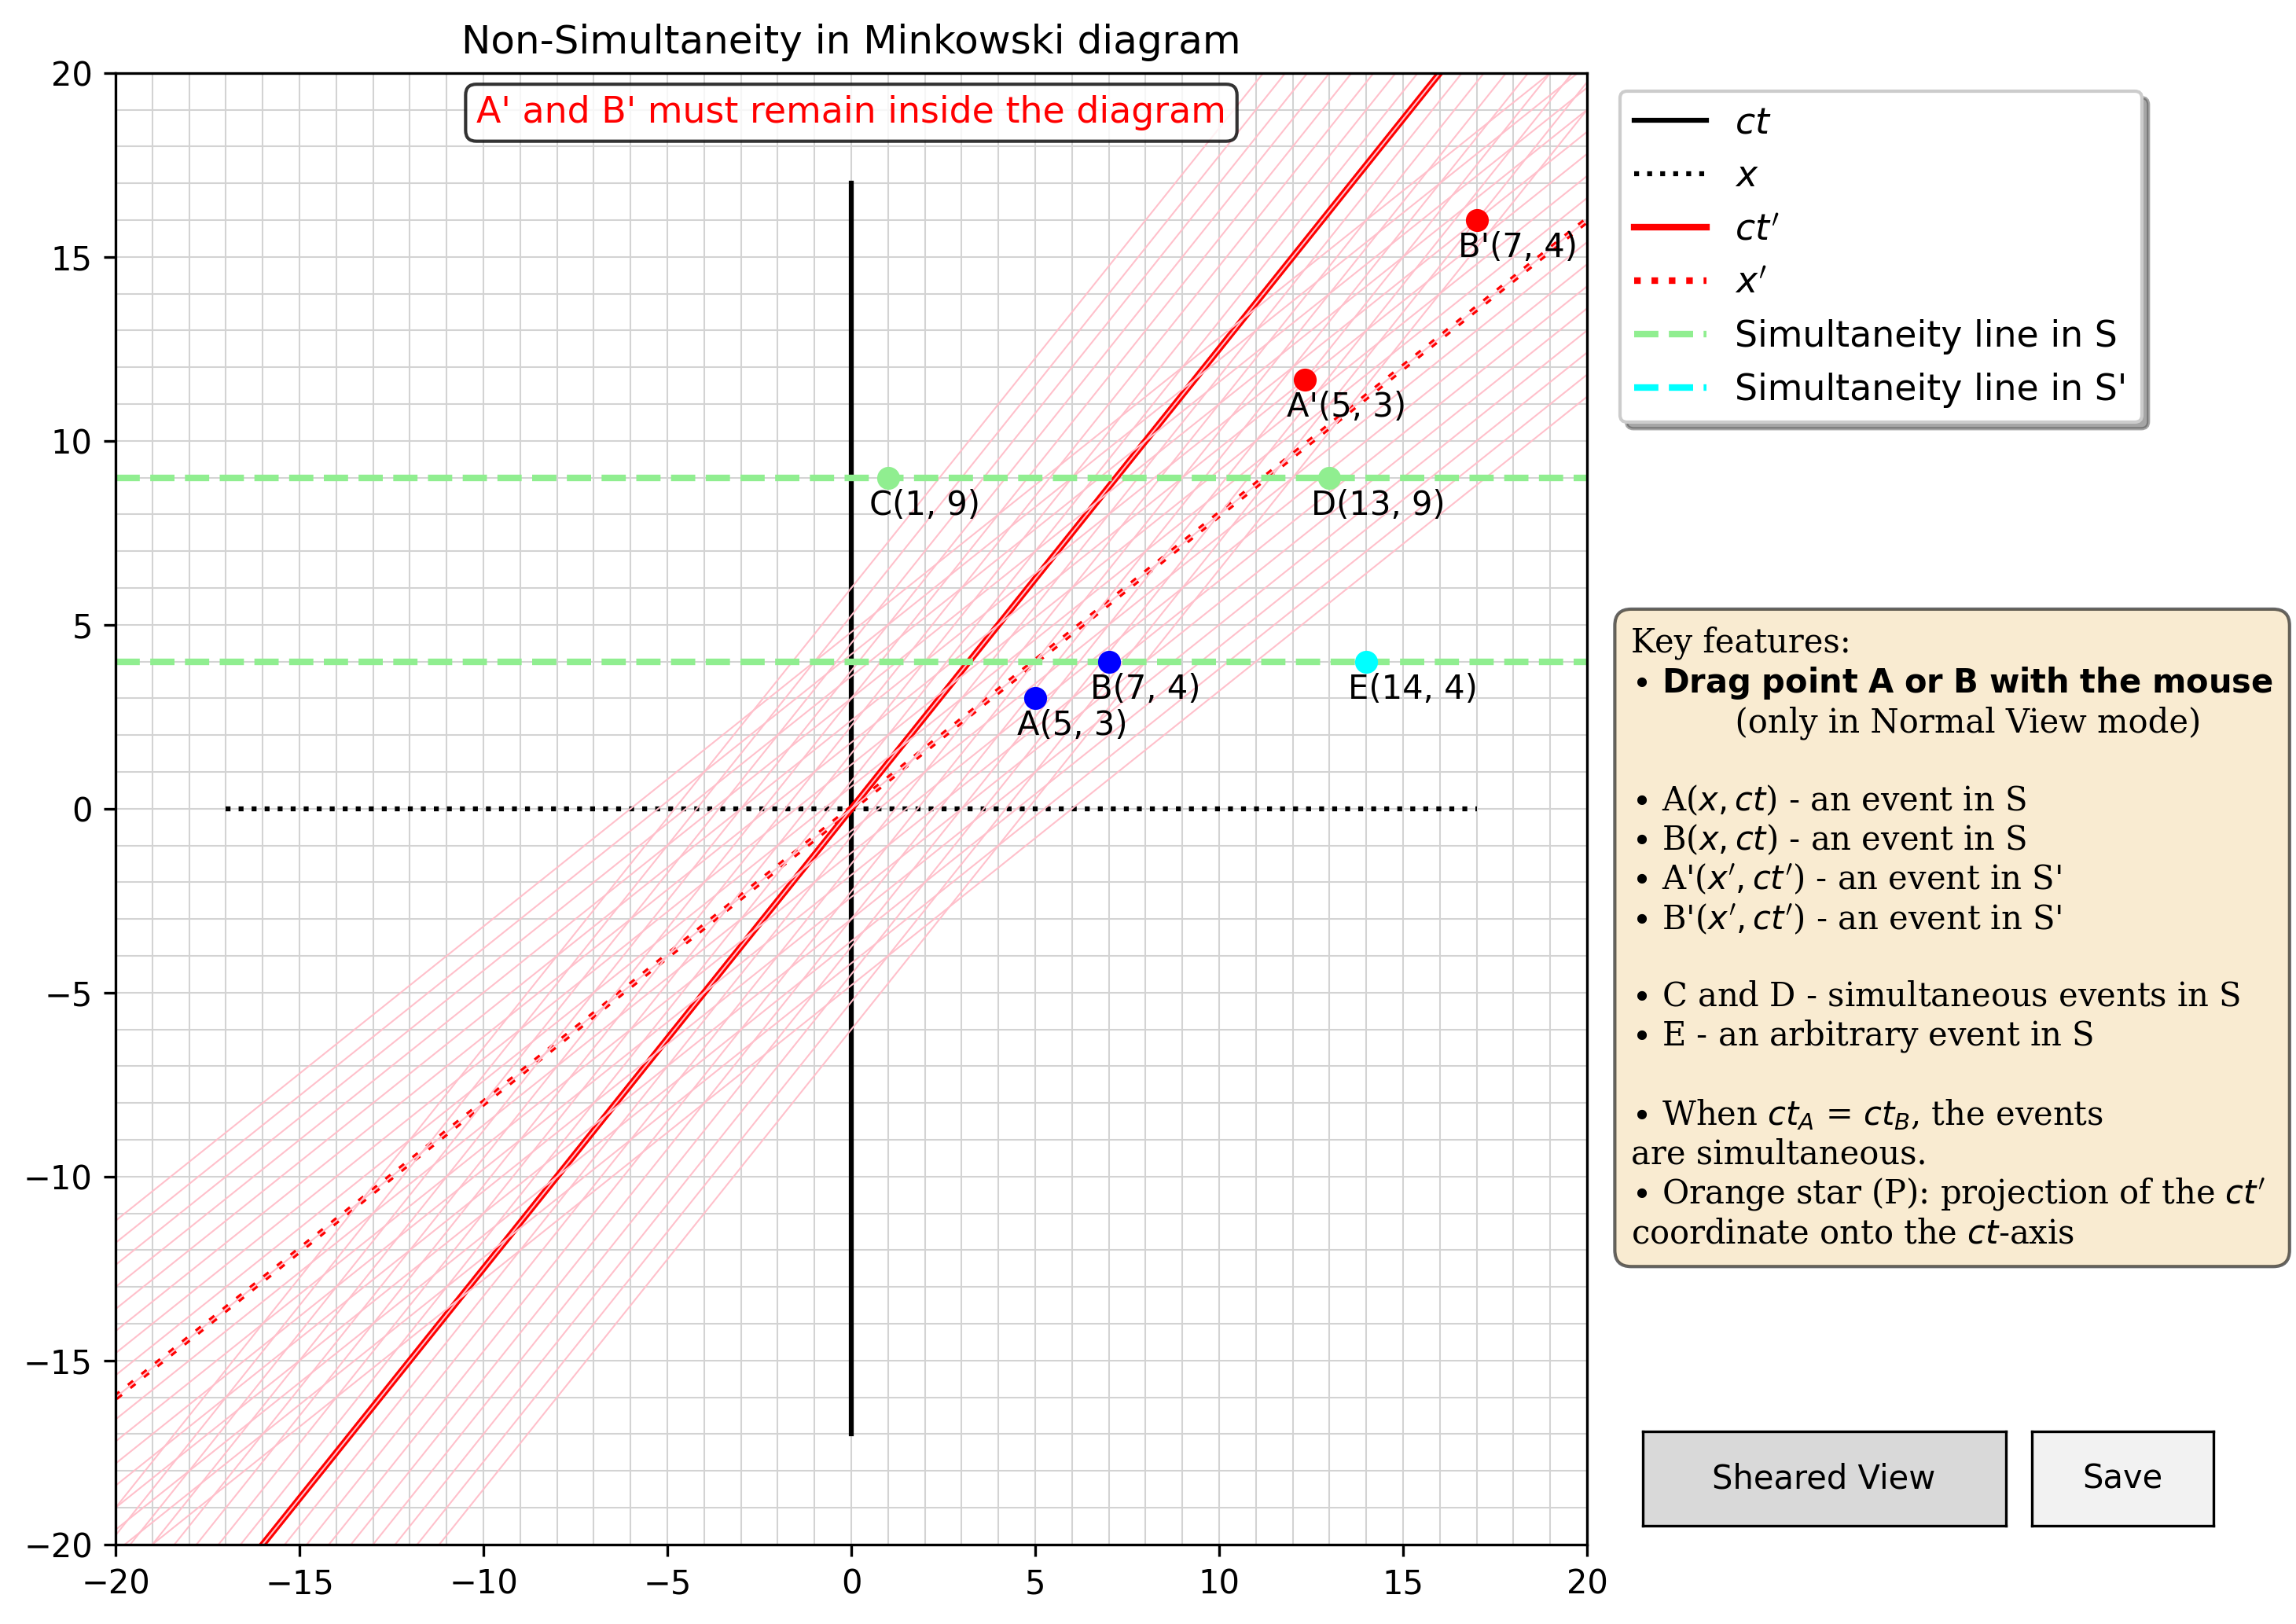
\includegraphics[width=0.7\textwidth]{figure3.png}
			\caption{Lorentz-consistent Minkowski diagram illustrating two distinct events with frame-dependent coordinate assignments}
			\label{fig3}
		\end{figure}
To illustrate the distinction more clearly, consider two events, shown in Fig.~\ref{fig3}. Events A and B are specified in S, while A' and B' denote their corresponding representations in S', obtained via mapping between frames. These pairs correspond to the same physical events but differ in their coordinate descriptions.

In this configuration, the events are not simultaneous in either frame.
If the coordinates of one event in S are adjusted so that it lies on the same simultaneity line as the other, its counterpart in S' acquires different coordinates and becomes simultaneous with the corresponding event in that frame, as illustrated in Fig.~\ref{fig4}.
		\begin{figure}[h]
			\centering
			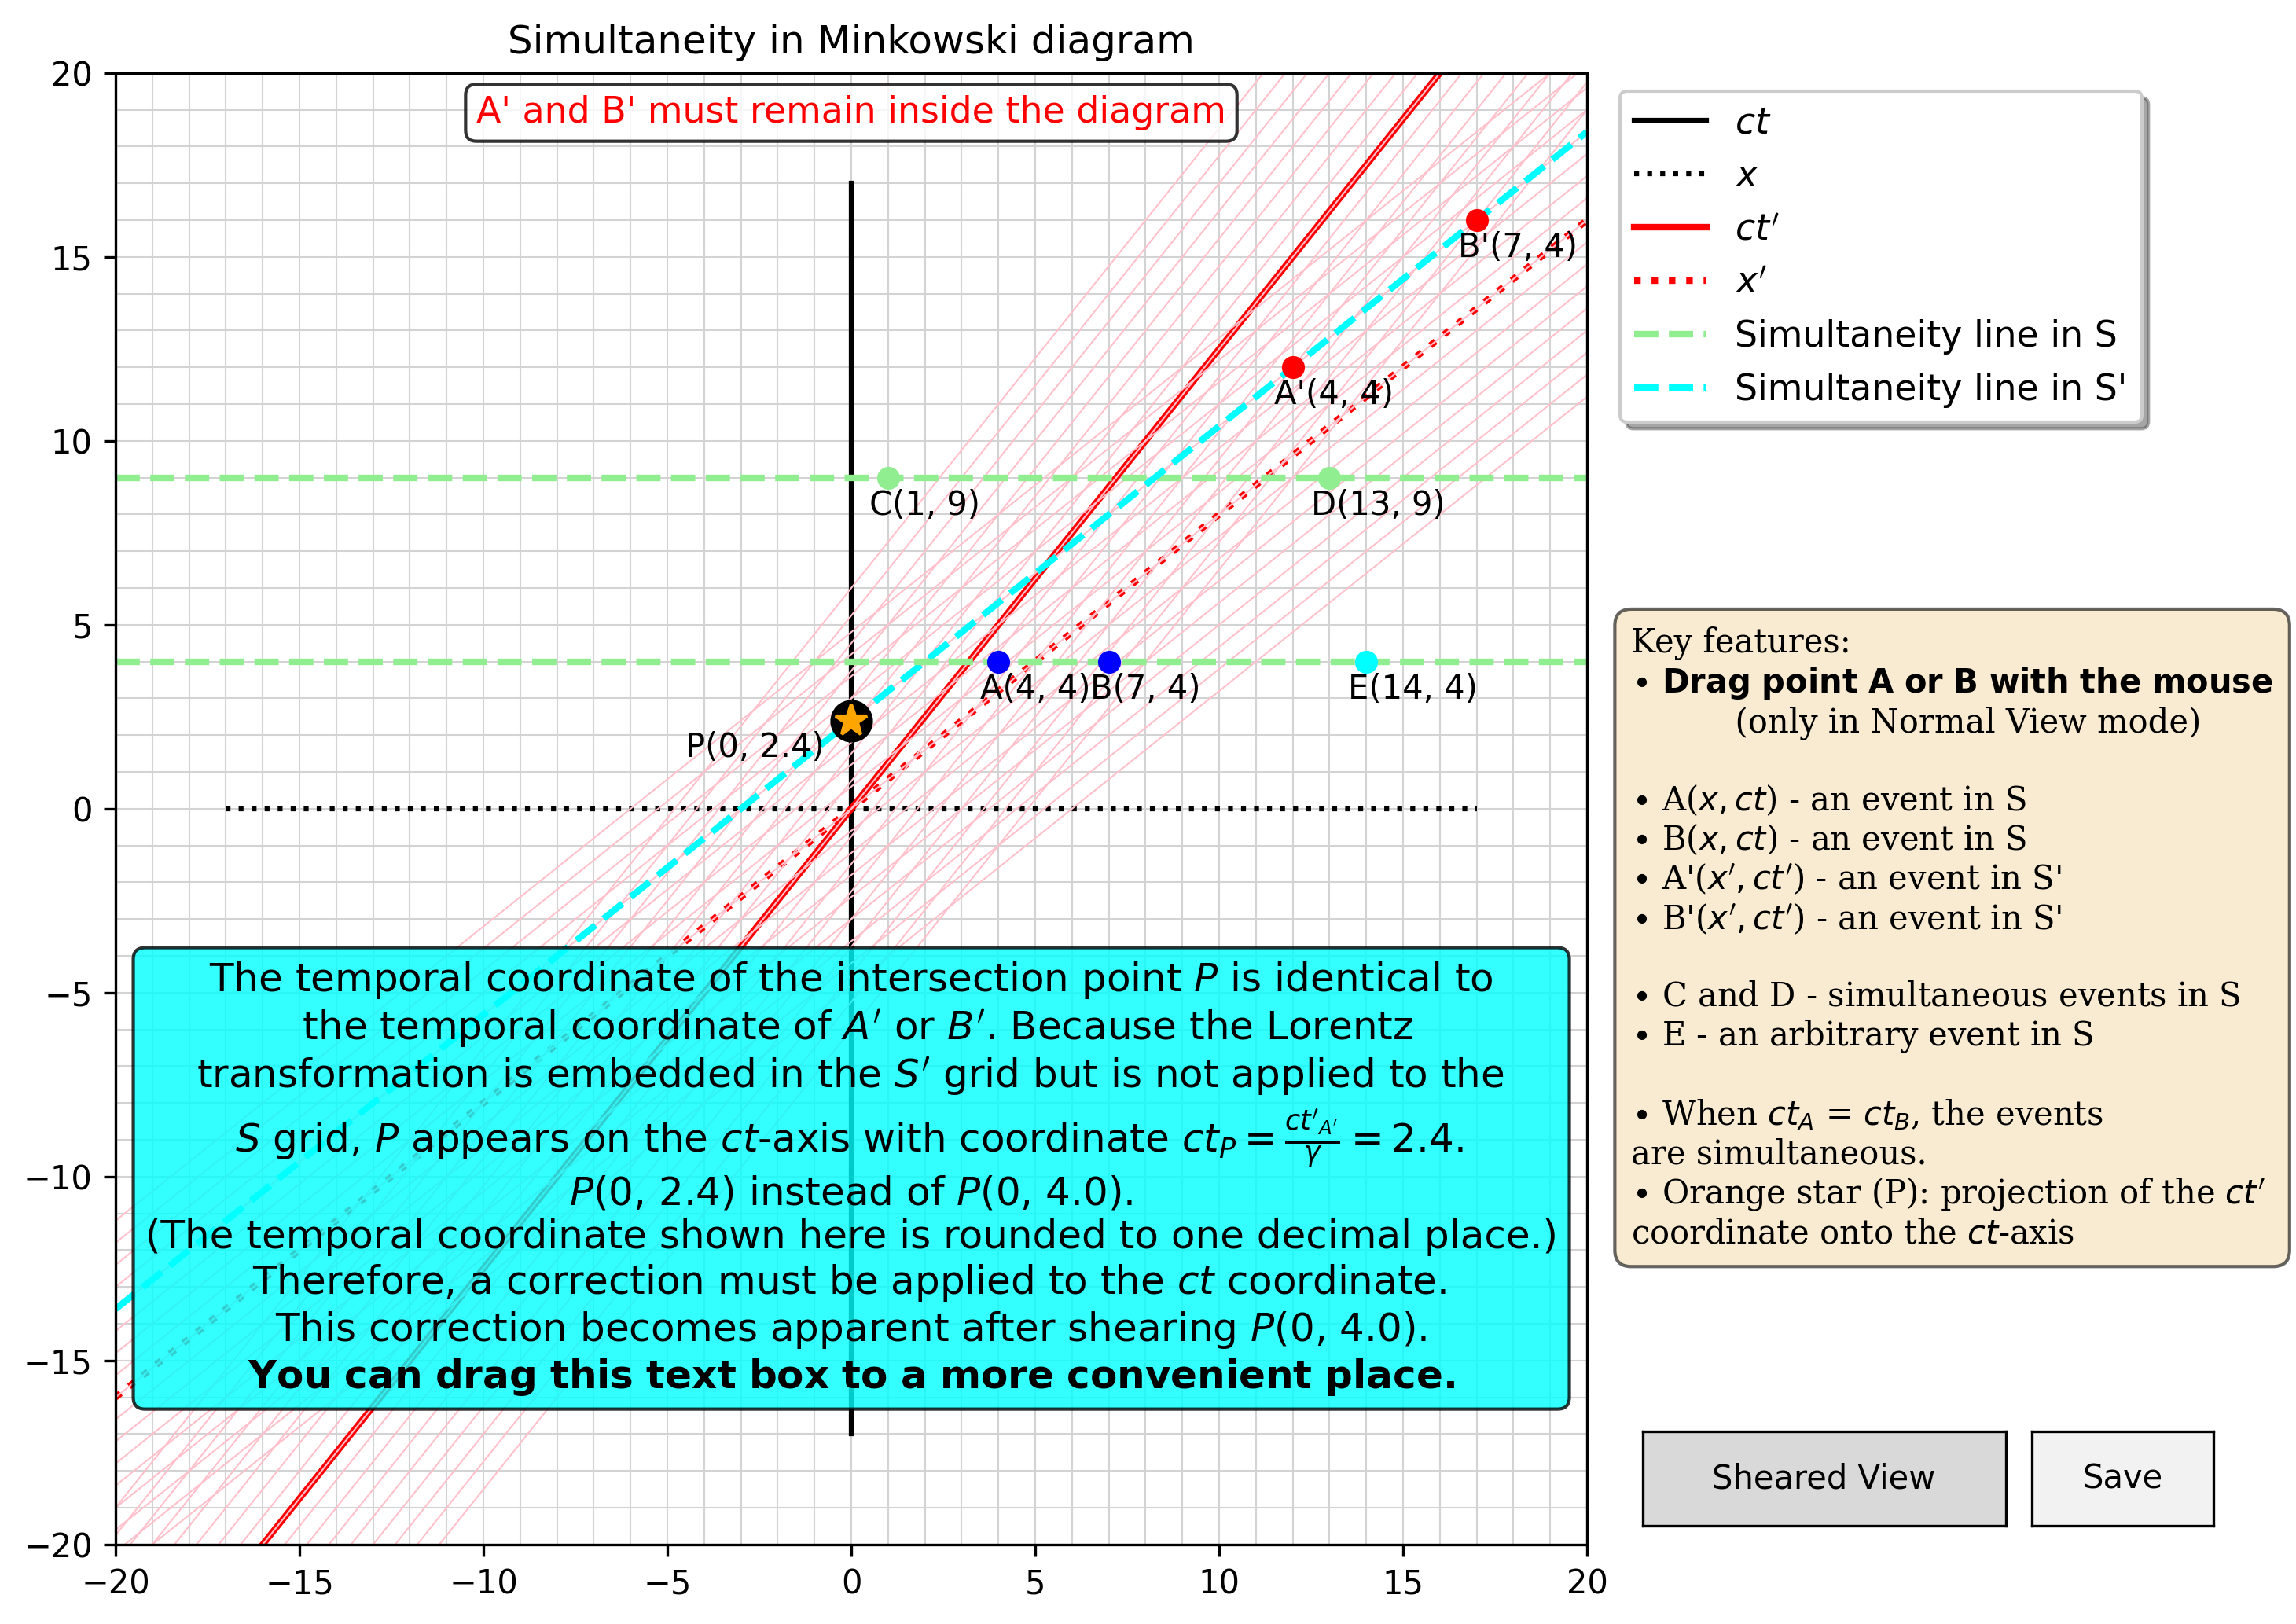
\includegraphics[width=0.7\textwidth]{figure4.png}
			\caption{Lorentz-consistent Minkowski diagram illustrating how coordinate reassignment changes simultaneity relations between events}
			\label{fig4}
		\end{figure}
An interactive Python implementation was developed to facilitate visualisation of these coordinate transformations and simultaneity relations. The code used to generate the figures is available in the archived repository (\texttt{src/figure4.py}).

However, since the Lorentz transformation factor is effectively embedded in the structure of the moving inertial frame, the coordinate relationships are preserved, and the physical identity of the spacetime event remains invariant, even though the local units of measurement may differ between frames. 

 Fig.~\ref{fig2} is drawn from the perspective of S; therefore, to interpret it from S', the diagram must be sheared so that the $ct'$ axis is rendered vertical, preserving internal consistency.
Applying the corresponding transformation yields Fig.~\ref{fig5}.
		\begin{figure}[h]
			\centering
			
\includegraphics[width=0.9\textwidth]{figure5.png}
			\caption{Lorentz-consistent Minkowski diagram illustrating the transformed simultaneity structure for v = 0.8c.}\label{fig5}
		\end{figure}
Since simultaneity is fundamentally a temporal concept, any line perpendicular to the vertical time axis defines a simultaneity plane. In this representation, points P and T lie on the same horizontal line, indicating that they correspond to the same event. Moreover, the coordinate time associated with the $ct$ axis appears dilated when viewed from the non-inertial frame, with $ct'_5 < ct_5$, while the spatial units in S' are contracted compared with those in S, in agreement with the predictions of Special Relativity. This difference reflects the distinction between coordinate time and elapsed proper time, which underlies the standard interpretation of "time dilation".
	\subsection{The standard presentation and its limitations}\label{subsec2_2}
		The classic thought experiment involving a moving train struck by lightning, first derived by Einstein (1905) \cite{einstein1905} is frequently employed to illustrate the relativity of simultaneity. While this scenario successfully demonstrates how observers in different reference frames may perceive events differently, it may obscure the underlying physical reality.

This paper argues that part of the apparent disagreement between observers arises from inconsistent identification of reference points in addition to the standard relativity of simultaneity. When reference points are chosen carefully across both inertial and non-inertial frames (and when physical verification conditions are met) all observers can consistently compare the same physical events once the reference frame and transformation procedure are clearly specified.
	\subsection{A refined scenario}\label{subsec2_3}
		Consider a modified version of the train scenario: A train moves along a track at constant velocity. Two lightning strikes occur: a red strike on the left-hand side (points A' on the train, A on the tracks) and a green strike on the right-hand side (points B' on the train, B on the tracks). For simplicity, we assume the lightning passes through gaps between carriages, leaving marks on both the train and the tracks (Fig.~\ref{fig6}).
		\begin{figure}[h]
			\centering
			
\includegraphics[width=0.9\textwidth]{figure6.png}
			\caption{A train is struck by two lightning bolts in the order RA’A–GB’B}\label{fig6}
		\end{figure}

		\textbf{Verification conditions:}
 	For simultaneity to be established, three conditions must be satisfied:
		\begin{enumerate}
			\item Both strikes leave marks on both the train and the tracks.
			\item The order of marks is consistent: Red aligns with A' and A, and Green aligns with B' and B.
			\item The transformed length A’B' must relate to the original length AB via Lorentz transformation.
		\end{enumerate}
  		\textbf{Note:}
It is crucial to understand how each observer perceives these lengths:

		\textbf{a) From the platform observer's (P)} rest frame: The train is moving at constant velocity. Consequently, the length of a carriage at rest ($L_0$) appears contracted to 
		\begin{equation*}
  			L'=\frac{L_0}{\gamma}
		\end{equation*}
For P, the distance AB on the tracks is merely the spatial projection of the segment A'B' on the train. Therefore, P measures AB = A'B' = L'.

		\textbf{b) From the train observer's (T)} rest frame: The observer is at rest relative to the carriage, so the carriage retains its proper length, $L_0$ . Thus, T measures A'B' = $L_0$. However, for T, the track segment AB is moving, and thus appears contracted. Consequently, T measures 
		\begin{equation*}
			AB = \frac{A'B'}{\gamma} = \frac{L_0}{\gamma}
		\end{equation*}
		\textbf{Conclusion:} The third condition is perceived differently in each frame:
		\begin{itemize}
			\item	For P: AB = A'B'
			\item	For T: 
  				\begin{equation*}
					AB = \frac{A'B'}{\gamma}
				\end{equation*}
		\end{itemize}
	\subsection{Observer perspectives}\label{subsec2_4}
		\textbf{Platform observer (P):} The observer on the platform perceives the strikes as simultaneous. This can be verified because:
			\begin{enumerate}
				\item Both strikes hit the train and the tracks → simultaneity
				\item The order of marks is RA’A—GB'B → simultaneity
				\item AB = A'B' → simultaneity
			\end{enumerate}
		\textbf{Train observer (T):} The observer on the train may initially perceive the strikes in a different order due to their motion. However, this perception may reflect a distortion caused by motion rather than a fundamental difference in simultaneity, when the same verification conditions are applied:
			\begin{enumerate}
				\item Both strikes hit the train and the tracks → simultaneity
				\item The order of marks is RA’A—GB'B → simultaneity
				\item 
    					\begin{equation*}
  						AB=\frac{A'B'}{\gamma} \to simultaneity
    					\end{equation*}
			\end{enumerate}
	As long as these conditions are satisfied, both observers can consistently identify the same physical events and compare them without contradiction, even though their coordinate descriptions may differ.
	
	\subsection{Illustrative examples:}\label{subsec2_5}
		\textbf{Example 1:} Green lightning hits first at points B’ and B; then red lightning hits the train at point A’. Because the strike does not pass through the gap between carriages, the mark appears only on the train, not on the tracks (Fig.~\ref{fig7}).
			\begin{figure}[h]
				\centering
				
\includegraphics[width=0.9\textwidth]{figure7.png}
				\caption{A train is struck by two lightning bolts in the order RA’–GB’B.}\label{fig7}
			\end{figure}
			\begin{enumerate}
				\item Both strikes hit the train, not the tracks → non-simultaneity
				\item Order: RA’—GB’B → non-simultaneity
				\item $AB \not= A'B'$ for P, and for T:
      					\begin{equation*}
  						AB\not=\frac{A'B'}{\gamma} \to non-simultaneity
      					\end{equation*}
			\end{enumerate}
		\textbf{Example 2:} Red lightning strikes first at points B’ (on the train) and A (on the track); the train moves, and then green lightning hits points A’ (on the train) and B (on the track) (Fig.~\ref{fig8}).
			\begin{figure}[h]
				\centering
				
\includegraphics[width=0.9\textwidth]{figure8.png}
				\caption{A train is struck by two lightning bolts in the order RB’A–GA’B.}\label{fig8}
			\end{figure}
			\begin{enumerate}
				\item Both strikes hit the train and the tracks
				\item Order:  RB’A–GA’B → non-simultaneity
				\item $AB = A'B'$ for P, and for T:
      					\begin{equation*}
  						AB =\frac{A'B'}{\gamma}
      					\end{equation*}
			\end{enumerate}
		\textbf{Rule:} Any combination of RB’, RB, GA’, or GA will lead to non-simultaneity (where RB and GA means the strikes were before or after the train).

		\textbf{Example 3:} First, green lightning strikes points B' (on the train) and B (on the tracks) simultaneously in the ground frame, occurring just after carriage \#1. As the train moves, red lightning strikes A' (on the train) and A (on the tracks, just after carriage \#3). Consequently, the distance A'B'—measured within the moving train frame—has expanded from one carriage to two (Fig.~\ref{fig9}).
			\begin{figure}[h]
				\centering
				
\includegraphics[width=0.9\textwidth]{figure9.png}
				\caption{A train is struck by two lightning bolts in the order RA’A–GB’B (non-simultaneous)}\label{fig9}
			\end{figure}
			\begin{enumerate}
				\item Both strikes hit the train and the tracks
				\item Order: RA’A—GB’B
				\item $AB \not= A’B’$ for P, and for T:
   					\begin{equation*}
  						AB \not=\frac{A'B'}{\gamma} \to non-simultaneity
      					\end{equation*}
			\end{enumerate}
	\subsection{The role of reference points}\label{subsec2_6}
	The platform observer analyses reference points from both frames (A'B' from the moving frame and AB from the inertial frame) and therefore reaches a consistent conclusion about simultaneity.
	For the train observer, the situation differs: they initially analyse only points of reference from their own moving frame—A’, B'. To reach the same conclusion, they must either apply appropriate corrections when transferring measurements to the inertial frame or select reference points from both frames.
This process is analogous to unit conversion: just as one must convert centimetres to inches to compare lengths accurately, one must apply Lorentz transformations to compare temporal measurements across frames.
	While Special Relativity remains valid within non-inertial frames, proper transformations are required when transferring measurements to an inertial reference frame.
	\subsection{The Distinction Between "Now" and "Observation"}\label{subsec2_8}
A critical distinction must be made between the ontological present (the actual state of events occurring "now") and the epistemological delay (the time it takes for information to reach an observer).

	Consider two events separated by a vast distance. While they may occur simultaneously in the common comparison frame, an observer will only become aware of the distant event after a delay determined by the speed of light. This delay creates the illusion that the distant event belongs to the "past", even though it is occurring in the frame-defined simultaneity.

		\textbf{Analogy:} Imagine calling a friend and asking them to mail an original document. Your friend states, "I am sending it to you now", while standing at the post office. In the absolute sense, the act of mailing and your receipt of the information are simultaneous in the timeline of the universe. 

However, you will not be "updated" about this event until the physical mail arrives days later.
	This illustrates that the plane of simultaneity (the set of events assigned the same coordinate time within a chosen reference frame) is fundamentally distinct from the observational hypersurface (the set of events we have received information about). The delay in receiving information does not negate the simultaneity of the event itself; it merely reflects the finite speed of signal transmission.

	This distinction provides a direct resolution to the Andromeda Paradox—as originally formulated by Rietdijk (1966) and Putnam (1967). In that thought experiment, two observers walking in opposite directions are said to have different "nows" regarding an event in the Andromeda galaxy (millions of light-years away). Under the standard interpretation, this implies that reality itself is fragmented.

However, under the Time vs. Duration framework, the now in Andromeda is a single event. The difference between the two observers is not in the existence of the event, but in their observational hypersurface. One observer's now slice intersects the light signal from Andromeda that left millions of years ago, while the other's intersects the same signal but slightly later.

	The "paradox" arises only when we confuse the arrival of the signal (observation) with the occurrence of the event (reality). Once we separate the two, causal coincidence is preserved, and the paradox dissolves.

\section{The Twin Paradox – Time vs. Duration}\label{sec3}
	\subsection{Distinguishing Time from Duration}\label{subsec3_1}
    	A primary source of confusion surrounding the twin paradox lies in the conflation of two distinct concepts: time—coordinate time—and duration—proper time. In spacetime, coordinate time functions as a spacetime coordinate analogous to the spatial coordinates  $x$, $y$, and $z$, while remaining physically distinguished by the metric signature.
	
	While we never directly measure $x$, $y$, or $z$ (we measure intervals $\Delta x$, $\Delta y$, and $\Delta z$) similarly, we do not measure time itself, but rather  $\Delta t$— the duration between two events.
	A crucial distinction emerges:
		\begin{itemize}
			\item Time—coordinate time—serves as the reference for all observers.
			\item Duration—proper time—depends on the geometry of the world-line and therefore differs for observers following different inertial or accelerated trajectories.
		\end{itemize}
    	This distinction parallels the relationship between mass and weight: mass remains constant regardless of gravitational environment, while weight varies with local conditions. The distinction between coordinate time and proper duration can clarify pedagogical misunderstandings of Special Relativity without challenging the theory's mathematical framework.

	\subsection{Mathematical framework}\label{subsec3_3}
Consider the following parameters for analysis:
		\begin{itemize}
			\item Speed: $v$ = 0.8c
			\item Distance (Earth to star, rest): 4 light-years
			\item Round-trip distance ($L_0$): 8 light-years
		\end{itemize}
In the Inertial Frame (Earth):
		\begin{equation*}
  			\Delta t_0 = \frac{L_0}{v} = \frac{8}{0.8} = 10 \text{ years}
		\end{equation*}
Lorentz factor:
		\begin{equation*}
  			\gamma = \frac{1}{\sqrt{1 - \frac{v^2}{c^2}}} = \frac{1}{\sqrt{1 - 0.64}} = 1.67
		\end{equation*}
Length Contraction (moving inertial frame):
		\begin{equation*}
  			L' = \frac{L_0}{\gamma} = \frac{8}{1.67} = 4.8 \text{ light-years}
		\end{equation*}
Proper Duration (Traveller):
		\begin{equation*}
  			\tau = \frac{\Delta t_0}{\gamma} = \frac{10}{1.67} \approx 6 \text{ years}
		\end{equation*}
Duration Difference:
		\begin{equation*}
  			D_{difference} = \Delta t_0 - \tau = 10 - 6 = 4 \text{ years}
		\end{equation*}
	\subsection{Velocity consistency check}\label{subsec3_4}
		From the traveller's perspective, the velocity calculation must remain consistent:
		\begin{equation*}
  			v = \frac{L'}{\tau} = \frac{4.8}{6} = 0.8c
		\end{equation*}
	\subsection{The return to rest frame}\label{subsec3_5}
The complexity arises when the spaceship returns to Earth and becomes non-moving again. At that point, the distance between Earth and the star returns to its original value—8 light-years (round-trip). The traveller's clock records only 6 years of proper duration, but this does not imply that "time itself" has been permanently altered. The traveller's clock does not recover the elapsed coordinate time. Once motion ceases and both twins are again in rest frames, physical quantities such as distance and time are consistently defined—there is no paradox.

	\subsection{ Addressing common misconceptions}\label{subsec3_6}
		\textbf{Incorrect calculation (after returning to the rest frame):}
			\begin{equation*}
  				v = \frac{L_0}{\tau} = \frac{8}{6} = 1.33c 
			\end{equation*}
	This calculation erroneously transfers untransformed measurements ($\tau$) from an moving-inertial frame to an inertial frame, yielding a superluminal velocity ($v > c$) that contradicts the fundamental postulates of Special Relativity. Years measured in an non-inertial frame are not directly equivalent to years in an inertial frame; each frame possesses its own consistent system of measurement. Upon the restoration of the length to its rest value in the inertial frame, the measured duration must likewise revert to its corresponding inertial-frame value, the two quantities are inextricably linked by the Lorentz transformation.

		\textbf{Correct calculation (after returning to the rest frame):}
			\begin{equation*}
  				v = \frac{L_0}{\tau \times \gamma} = \frac{8}{6 \times 1.67} = \frac{8}{10} = 0.8c
			\end{equation*}
			\begin{equation*}
  				\Delta t_{Spaceship} = \frac{\gamma \times L'}{v} = \frac{L_0}{v}=\frac{8}{0.8} = 10 					\text{ years}
			\end{equation*}

	\subsection{The limit as v approaches c}\label{subsec3_7}
		As velocity approaches the speed of light: 
		\begin{equation*}
  			\lim_{v \to c^-} \gamma = \infty
		\end{equation*}
		\begin{equation*}
  			\lim_{v \to c^-} \tau = \lim_{v \to c^-} \frac{\Delta t_0}{\gamma} = 0
		\end{equation*}
		\begin{equation*}
  			\lim_{v \to c^-} L' = \lim_{v \to c^-} \frac{L_0}{\gamma} = 0
		\end{equation*}
The limit:
		\begin{equation*}
  			\lim_{v \to c^-} \tau = 0  
		\end{equation*}
should not be interpreted as light "stopping" or having no duration. Photons do not possess a rest frame in Special Relativity. We are simply evaluating the mathematical limit of the proper time expression using the Lorentz transformation, without requiring a physical rest frame for the photon.
		\begin{equation*}
  			v = \frac{L_0}{\tau \times \gamma} = \frac{L_0}{\Delta t_0}
		\end{equation*}
		\begin{equation*}
  			\lim_{v \to c} v = \lim_{v \to c} \frac{L_0}{\Delta t_0} = \frac{L_0}{\frac{L_0} c} = \frac{L_0} {L_0} \times c = c
		\end{equation*}
The vanishing of proper duration ($\tau \to 0$) and contracted length ($L' \to 0$) does not imply a breakdown of physics, but rather that the "relative" measurements collapse to zero while the "absolute" coordinate relationship $L_0 = \Delta t_0 \times c$ remains intact.
	This supports the paper's thesis that coordinate time and simultaneity serve as the stable, common comparison frame, while duration and length are relative measurements subject to transformation.
	Attempting to substitute numerical values directly into expressions involving infinity leads to meaningless results. Instead, algebraic simplification reveals the correct behaviour:
	To find the coordinate time in the limit as $v \to c$, we first simplify the algebraic expression before applying the limit:
		\begin{equation*}
  			\Delta t_{\text{Light}} = \frac{\gamma \times L'}{c} = \frac{\gamma \times \frac{L_0}{\gamma}}{c} = \frac{L_0}{c}
		\end{equation*}
  Now, taking the limit as $v \to c$
		\begin{equation*}
  			\lim_{v \to c} \Delta t_{\text{Light}} = \frac{L_0}{c} = \frac{8 \text{ ly}}{c} = 8 \text{ years}
		\end{equation*}
  	This demonstrates that while $\gamma \to \infty$ and $L' \to 0$ individually, their product remains finite and equal to the rest distance $L_0$, preserving the consistency of the speed of light.

	\subsection{Photons and proper time}\label{subsec3_8}
		The claim that "photons don't experience time" requires careful interpretation. From a photon's perspective, its proper time is zero.
However, when compared with other reference frames, corrections must be applied. When a photon is absorbed, its proper time returns to a non-zero value relative to the absorbing frame.
	If proper time were absolute, no corrections would be necessary. The fact that corrections are required indicates that proper time is relative to the observer's state of motion.

\section{Spacetime and the Nature of Time}\label{sec4}
	\subsection{The four-dimensional framework}\label{subsec4_1}
	We inhabit a four-dimensional universe, comprising three spatial dimensions and one temporal dimension, a concept formalised by Minkowski \cite{minkowski1908}. However, our habitual treatment of spacetime as merely three-dimensional creates conceptual difficulties when attempting to grasp its true nature. Einstein's statement that 'time is relative to the observer' \cite{einstein1905} refers to the dependence of time measurements on the observer's frame of reference—not to the subjectivity of spacetime itself. This relativity applies to all physical quantities, not exclusively to time.

	Einstein distinguished between two kinds of time: coordinate time and proper time. Over the past century, translation nuances and interpretive drift have rendered these terms sources of ongoing confusion.
	\subsection{Time as a dimension}\label{subsec4_2}
	A common difficulty in fully grasping Special Relativity arises from attempting to understand time dilation before establishing a precise definition of time itself. 
	Time functions as a dimension analogous to the $x$, $y$, and $z$ axes, yet with a distinctive characteristic: while spatial axes are static, the temporal axis is inherently dynamic. We can remain stationary along spatial directions, but remaining still in time is impossible.
	The infinite nature of these axes means we cannot measure them directly. We establish reference points (coordinates) and measure the intervals between them: $\Delta x$, $\Delta y$, and $\Delta z$. Thus, we measure duration—$\Delta t$—between two events on the temporal axis, not time itself.

The temporal axis is directional and continuous, always progressing forward — we cannot return to a previously occupied point on this axis as we can with spatial coordinates.
	Since time is an integral component of the spacetime structure, any transformation affecting one dimension must proportionally affect the others, much like the arms of a pantograph. If the arms of a pantograph did not move in strict proportion, the resulting image would be distorted rather than a scaled replica. This principle is confirmed by Special Relativity: in an accelerated frame, both spatial length and proper duration ($\tau$) contract by the same factor ($\gamma$), thereby preserving the geometric proportionality of spacetime. If one changed without the other (i.e., if $\tau$ did not return to its rest value—as length does—when the traveller twin returns), the "shape" of physics (the speed of light, causality) would break.
	\subsection{Coordinate Time vs. Proper Duration}\label{subsec4_3}
	When Einstein stated that "time is relative'" he likely referred to proper time. This terminology is somewhat misleading, as "proper" suggests something to be taken for granted. More precise alternatives might include "relative time", "observer's time", or "proper duration".

	Coordinate time serves as the universal reference for all observers; all calculations reference it. From this perspective, coordinate time functions as the temporal axis itself and should be considered common comparison frame.

	Proper duration, by contrast, is relative to the observer and can be affected by acceleration and gravity. This is why duration is not continuous in the same way as coordinate time, and why Einstein described proper time as relative.
	
	Special Relativity asserts that no reference frame is preferred—all observers are equally valid within their own frames. However, meaningful comparison of events or measurements between frames requires agreement on a common reference frame for performing transformations. Without such consensus—for instance, without agreeing on which train is under discussion—comparisons become impossible. In this operational sense, the agreed-upon frame assumes the role of an common comparison frame with frame-defined simultaneity values and coordinates.
	
	\subsection{Clocks and measurement}\label{subsec4_4}
	Most clocks measure duration in relation to distance—pendulums, light beams between sensors, crystal vibrations, atomic oscillations. If the distance changes due to acceleration, the measured duration changes accordingly. A clock unaffected by acceleration would measure coordinate time directly; however, all practical clocks are susceptible to velocity and gravitational effects. Thus, clocks do not measure time itself, but rather the duration traversed through spacetime since a reference point was established. This explains why clocks reset every 12/24 hours and years every 365 days without causing problems—the resets are conventions, not reflections of time itself changing.

	To visualise the distinction between time and duration, consider a magnetic tape recording. Imagine a song recorded on a magnetic tape, starting at index A and ending at index B. The indices on the tape represent the operationally invariant coordinate time: the song always begins at A and ends at B, regardless of how it is played.

However, the duration of the song depends on the playback speed. If we play the tape faster, the song finishes in less time; if slower, it takes longer. This change in playback speed is analogous to time dilation: the "duration" measured by a moving clock changes, but the underlying "tape" (the spacetime interval) remains fixed. Crucially, to truly “stretch time” (that is, alter the indices themselves), one would have to physically stretch the magnetic tape, thereby destroying the recording; thus, the proportions must be preserved.

This illustrates that while duration is relative and variable, time (the coordinate dimension) is operationally invariant. Changing the playback speed does not alter the song's content or its position on the tape; it only alters the rate at which we traverse it.

	\subsection{Visualising spacetime}\label{subsec4_5}
	Representing four-dimensional spacetime on paper is inherently limited. Standard representations of spacetime utilise three orthogonal spatial axes ($x, y, z$) alongside a vertical time axis, frequently parallel to the $z$-axis. This alignment, however, risks ambiguity by binding the temporal and spatial $z$ dimensions. To mitigate this, Fig.~\ref{fig10} adopts a superior representation in which the time axis is distinctly marked in red.
		\begin{figure}[h]
			\centering
			
\includegraphics[width=1.2\textwidth]{figure10.png}
			\caption{3D Spacetime}\label{fig10}
		\end{figure}
Employing a distinct red time axis alongside all three spatial axes eliminates the misconception that spatial motion necessarily entails temporal distancing. This fallacy emerges solely in single-axis temporal representations.

Each "tick" of time represents a new configuration of space at that moment. These configurations join together like pages in a book or frames on celluloid film, each bearing a timestamp representing the state of space at that instant. When two events occur simultaneously at different spatial locations, they share the same temporal coordinate—hence the term "simultaneous".  As noted earlier, the coordinate values of an event remain the same, even when the local units of measurement differ between frames.

Since time progresses continuously, we do not "move" through time in the spatial sense; rather, we remain at a fixed point on the temporal axis while new spatial configurations are generated around us. The "present" exists only as an infinitesimal moment before the next spatial configuration is created. In this sense, while we exist in the present (at t = 0), we live in the past due to the delay in receiving information.

	It is crucial to distinguish the temporal dimension (t-axis) from clock measurements. Coordinates on the t-axis do not signify the passage of time or discrete "ticks"; they serve merely as a framework for tracking the relative duration intervals measured by clocks. This distinction resolves the confusion at the heart of the Rietdijk–Putnam argument. Often interpreted as proof of the "Block Universe" (Eternalism), this conclusion relies on conflating observational delay with ontological reality \cite{rietdijk1966, putnam1967}. Because we cannot instantly agree on when we see now, we mistakenly assume now itself is relative.

	However, now exists absolutely; the delay is merely in our perception. By separating the operationally invariant temporal dimension from the relative measurement of duration, we can retain the mathematical success of Special Relativity while preserving an common comparison frame (Presentism), thereby resolving paradoxes without accepting the fragmentation of reality.
	Thus, to accurately reflect the "Presentist" view where the future is uncreated, the spacetime diagram should appear as in Fig.~\ref{fig11}.
		\begin{figure}[h]
			\centering
			
\includegraphics[width=1\textwidth]{figure11.png}
			\caption{3D Spacetime: Present \& Past Only (Future Not Created)}\label{fig11}
		\end{figure}
	\subsection{An analogy for simultaneity}\label{subsec4_6}
	Consider a book where two words, A and B, appear on the same page (page 9). Their creation timestamp is identical—simultaneity frame. This establishes their simultaneity within the book's structure—spacetime. 
	If a reader browses the book randomly or backwards (observer frame-dependent), they may encounter a word B on page 35 and a word A on page 20. This creates the illusion that the words appeared at different times ($t_{35}$) and ($t_{20}$). However, these timestamps represent the moment of observation, not the moment of creation. By returning to the correct reference point—the first page—and verifying that both words share the original timestamp $t_9$, we confirm their simultaneity. It is logically impossible for two distinct events to share an identical creation timestamp unless they are, by definition, simultaneous—the same simultaneity frame. Even if the words reappear later on the same page ($t_{30}$), this does not alter the simultaneity frame established at the moment of their creation ($t_9$).

Thus, the simultaneity frame is preserved, even when compared against itself across different instances of observation, while the observation of events is frame-dependent.

The two must not be conflated.

\section{Reconciling with Standard Interpretations}\label{sec5}
	\subsection{The standard view:}\label{subsec5_1}
	Relativity of Simultaneity and Time: In the standard formulation of Special Relativity, the relativity of simultaneity is a fundamental consequence derived directly from the constancy of the speed of light. According to this view, there is no universal now; events simultaneous in one inertial frame are generally not simultaneous in another. Furthermore, standard pedagogy treats proper time ($\tau$) as the invariant spacetime interval—the "true" time experienced by an observer—while coordinate time (t) is viewed as frame-dependent and relative. The "twin paradox" is traditionally resolved by noting that the travelling twin undergoes acceleration, breaking the symmetry between the two frames \cite{taylor1992}, resulting in a genuine difference in the accumulated proper time along their respective world-lines.

The dominant view in modern physics, often called Eternalism or the Block Universe, is argued by Brown \cite{brown2005} and Maudlin \cite{maudlin2012}. The debate between Eternalism and Presentism is the philosophical cornerstone of the interpretation of Special Relativity. 

		\textbf{Eternalism}, the dominant view in modern physics, posits that past, present, and future events all exist equally in a static four-dimensional manifold. This view is often derived from the Rietdijk–Putnam argument, which claims that because simultaneity is relative, there is no unique now \cite{rietdijk1966, putnam1967}, and thus the entire timeline must exist simultaneously. In this framework, the "flow" of time is an illusion of consciousness.

		\textbf{Presentism}, conversely, asserts that only the present moment is real. The past no longer exists, and the future has not yet been created. This view aligns with our intuitive experience of time but has historically struggled to reconcile with the relativity of simultaneity.
	\subsection{The proposed clarification: Semantic distinction vs. Physical contradiction}\label{subsec5_2}
	This paper does not dispute the mathematical predictions of Special Relativity—the Lorentz transformations, the invariance of c, or the experimental verification of time dilation. Rather, it proposes that the interpretive framework often obscures the underlying geometry. Mermin notes that the apparent contradiction arises from conflating measurement with physical reality (or dimension) \cite{mermin1984}. We further suggest that it also stems from failing to identify the corresponding reference points in both frames simultaneously.
	\subsubsection{On simultaneity:}\label{subsubsec5_2_1}
While standard formulations of Special Relativity treat simultaneity as frame-dependent, this paper argues that physical coincidence—that is, two events occurring at the same time—must be evaluated within the common reference frame chosen by all observers for comparison. The "relativity" arises only when observers attempt to synchronise clocks across a distance without accounting for the finite propagation of signals and the specific reference points chosen. By insisting on verification conditions that involve marks in both frames—as in the refined train scenario—, we recover an common comparison frame of simultaneity for the events themselves, even if the clock readings differ.
	\subsubsection{On Time vs. Duration:}\label{subsubsec5_2_2}
	Standard texts often state "time is relative". This paper suggests a more precise phrasing: "measured duration is relative to the path through spacetime, while the temporal dimension itself is invariant under transformation". Since both inertial and non-inertial frames reside within the same spacetime, where there exists only one set of spatial and temporal dimensions ($x, y, z$, and $t$), they share the same underlying coordinate structure inherited from spacetime itself. The fact that each observer may choose, for convenience, to adopt a local coordinate system does not alter this physical unity. Just as the distance between two points on the map is fixed—absolute—but the odometer reading depends on the route taken—relative—, the temporal axis exists independently, while the "duration" measured by a clock depends on the clock's velocity and acceleration history.
	\subsubsection{On Eternalism vs. Presentism:}\label{subsubsec5_2_3}
	The framework proposed in this paper seeks to preserve the mathematical consistency of Special Relativity while offering an interpretation compatible with Presentist ontology. By distinguishing between coordinate time as the common spacetime parameter and proper duration as the observer-dependent physical measurement, we argue that:
		\begin{itemize}
			\item The relativity of simultaneity is a feature of reality, not a feature of measurement (how different observers slice the timeline).
			\item The coordinate time provides a unique, universal now that exists independently of the observer's state of motion.
			\item Within this interpretation, the future is not treated as a pre-existing region of the spacetime manifold awaiting discovery, but rather as the not-yet-realised extension of the time dimension, whose physical content emerges only through the progression of events.
 		\end{itemize}
	Thus, the "Block Universe" is revealed to be a misinterpretation of the geometry of spacetime. The geometry is real, but the "block" is not static; it is a growing manifold where the "present" is the leading edge of creation. This resolves the Andromeda Paradox not by fragmenting reality, but by acknowledging that while observers disagree on "when" they receive the signal, they agree on the "moment" the event occurred.
	\subsection{ Why this framework offers additional clarity: Adopting the distinction between common coordinate time and relative proper duration offers four specific pedagogical advantages:}\label{subsec5_3}
		\begin{itemize}
			\item Resolution of Intuitive Paradoxes: It removes the counter-intuitive notion that "time itself" slows down or that the future is not fixed. Instead, it frames the effect as a mechanical consequence of the path taken through a spacetime manifold.
			\item Consistency with Unit Conversion: It aligns relativistic corrections with familiar engineering concepts (like the Mars Climate Orbiter unit error) \cite{nasa1999}. Students can understand that transferring a measurement from an non-inertial frame to an inertial one requires a "conversion factor" ($\gamma$), rather than accepting that the physical laws themselves change.
 			\item Clarification of the Photon Limit: It provides a coherent explanation for the limit $v \to c$. In the standard view, the statement "photons experience no time" can seem mystical. In this framework, it is a straightforward mathematical limit where the duration measured along the light-like path vanishes, while the coordinate time—the distance travelled divided by c—remains well-defined and finite.
 			\item Reconciliation of Eternalism and Presentism: It resolves the philosophical deadlock between the Block Universe and the Growing Block. By treating coordinate time as the "absolute river" of existence and duration as the "speed" at which an observer traverses it, the framework allows for a Presentist interpretation of reality (where the future is uncreated) without violating the mathematical predictions of Special Relativity. This empowers students to discuss the nature of time philosophically without feeling forced to abandon the "reality" of the present moment.
		\end{itemize}
\section{ Conclusion on interpretation:}\label{sec6}
	\subsection{Conclusion on simultaneity}\label{subsec6_1}
		\begin{itemize}
			\item We should not conflate simultaneity with observing (simultaneity plane with observational slices through spacetime). 
			\item The framework presented above indicates that while observational slices through spacetime are frame-dependent, simultaneity is determined by the temporal coordinate ($t$), which maintains its value across different frames.	
			\item When reference points are chosen carefully and proper transformations are applied, all observers should agree on whether events are simultaneous. Apparent paradoxes arise not from the physics itself, but from inconsistent application of reference points or failure to apply necessary corrections when transferring measurements between frames.
			\item The spacetime diagram analysis assumes that the "vertical" axis represents the common temporal dimension, and the tilt represents the relative measurement of duration.
			\item By treating coordinate time as the common reference frame and proper duration as the relative measurement, we preserve the mathematical rigour of Special Relativity while eliminating the semantic ambiguities that lead to paradoxes. This approach does not replace Einstein's theory but rather refines the language used to describe it, making the transition from Newtonian intuition to relativistic reality more seamless.
		\end{itemize}
	\subsection{Conclusion on the Twin paradox}\label{subsec6_2}

	In many textbook treatments, the scenario is idealised by assuming that the travelling twin remains inertial over most of the trajectory, thereby simplifying the analysis. However, this approximation obscures the essential role of acceleration in enabling the return segment of the journey. The resulting asymmetry is often discussed in terms of a discontinuous “jump” in simultaneity \cite{rindler2006}; however, such a feature arises from the construction of piecewise inertial frames and does not represent a physical effect.
		\begin{itemize}
			\item As noted above, the formalism admits a more direct and transparent treatment without invoking this artefact ("the jump"). Moreover, in the limiting case of purely inertial motion, the proper time of the traveller coincides with that of the Earth-bound twin within a single inertial frame. These considerations underscore the importance of employing a physically consistent, rather than overly idealised, description of the scenario.
			\item As illustrated in Fig.~\ref{fig5}, the traveller's "proper time" is consistently shorter than the coordinate time ($\Delta t_0$) from the outset. This demonstrates that the observed "time dilation" is not a consequence of changing symmetries or reference frame transitions (such as turning around), but is an inherent effect of motion itself. Even if the traveller never returns to Earth and continues indefinitely in a straight line, their proper time remains shorter relative to $\Delta t_0$.
	Consequently, the coordinate time in the rest frame appears dilated from the perspective of the traveller's frame. It is this perceived expansion of the rest frame's coordinate time that gives rise to the term "time dilation", while in reality the duration—proper time—along the world-line is shorter. 
			\item More importantly, for both twins, the journey's duration and distance are divided into the same number of units—five units of time and four units of length per leg—despite their differing perceptions of those units. They employ different measurement systems, yet the coordinate values describing the events remain the same. Crucially, these two time intervals can still be compared and reconciled, provided we select reference points from both the inertial and moving inertial frames simultaneously, or perform the correct Lorentz transformation.
 			\item The traveller twin appears to have aged less \textbf{only} during the journey. \textbf{Once motion ends and both twins are again in rest frames, physical quantities are consistently defined.} The apparent age difference reflects the accumulated duration measured by the traveller's clock during the accelerated portions of the journey, not a fundamental alteration of time itself.
 			\item The main reason we struggle with the twin paradox is that we transfer raw measurements from an moving reference frame to an inertial frame without applying the proper transformations. Similarly, neglecting frame-to-frame corrections in relativistic scenarios leads to apparent paradoxes that dissolve under proper analysis. Moreover, drawing an incorrect or oversimplified grid for the moving inertial frame further amplifies the confusion.
		\end{itemize}
	\subsection{Conclusion on spacetime}\label{subsec6_3}
		\begin{itemize}
			\item We must distinguish between time and duration, choose reliable reference points when comparing events from inertial and non-inertial frames, or apply proper corrections. 
			\item When two events occur simultaneously, they possess their own reference frame—a simultaneity frame—which is preserved when transferred across different reference frames.
			\item While Special Relativity is one of the most rigorously tested theories in physics, it remains one of the most misunderstood. This confusion often arises from failing to distinguish between apparent distortions and fundamental changes.

Consider a stick submerged in water: it appears bent due to the refractive medium, but when the water is removed, the stick is revealed to be straight. Similarly, in Special Relativity, acceleration and velocity act as the "medium" that distorts measurements of length and duration. When motion ceases and the "medium" is removed, these measurements return to their inertial values. The traveller twin's clock records a shorter duration, but this is a record of the path taken through spacetime, not a fundamental alteration of the time dimension itself.

	This theoretical framework has practical implications for timekeeping instrumentation. A companion preprint—"Absolute Clock"—explores a clock design that minimises acceleration-sensitive measurements by counting photon emissions rather than relying on spatial oscillations. While this design does not claim to violate Special Relativity, it demonstrates the conceptual possibility of distinguishing between coordinate time and measured duration.
	
			\item Special Relativity remains fully valid during motion; however, attempting to retain untransformed measurements after the motion has ceased leads to apparent paradoxes, incorrect results, and conceptual confusion. 
			
			\item Ultimately, \textbf{no paradox remains once the data are complete and have been fully and consistently analysed.}
		\end{itemize}
\noindent\rule{\textwidth}{0.4pt}
\bibliography{references}
\end{document}
